\documentclass{scrartcl}
\usepackage[utf8]{inputenc}
\usepackage[swedish]{babel}
\usepackage{booktabs}
\usepackage{longtable}
\usepackage{tabu}
\usepackage{caption}
\usepackage{wasysym}
\usepackage{environ}
\usepackage{array}
\usepackage{graphicx}
\usepackage[table]{xcolor}

% utseende på labels
\captionsetup{margin=10pt,font=small,labelfont=bf,labelsep=period}

\author{\textbf{Magnus Johansson}\\
		magjo722@student.liu.se\\ \\
		\textbf{Rolf Lifvergren}\\
		rolli107@student.liu.se}

\title{Projektspecifikation}
\subtitle{Plattformsspel}

%% Kommando för kod inne i texten
%% Användningsexempel:
% \code{(define (square x) (* x x))}
\newcommand{\code}[1]%
{\texttt{#1}}

%% Kommando för ADT-tabell
%% Användningsexempel:
% \begin{adt-table}{\texttt{map\%}}{map-adt}
% 	render & canvas, dc & Ritar ut banan på skärmen
% \end{adt-table}
\NewEnviron{adt-table}[2]%
{\rowcolors{2}{gray!25}{white}
\begin{longtabu}{>{\bfseries}lp{4cm}X}
\hiderowcolors
\caption{#1}\label{#2}\\

\toprule
\textbf{Metod} & \textbf{Argument} & \textbf{Beskrivning} \\ 
\midrule
\endfirsthead

\hiderowcolors
\toprule
\multicolumn{3}{c}%
{\bfseries \tablename\ \thetable{}. (forts)} \\
\textbf{Metod} & \textbf{Argument} & \textbf{Beskrivning} \\ 
\midrule
\showrowcolors
\endhead

\hiderowcolors
\multicolumn{3}{r}%
{\bfseries(fortsätter på nästa sida)} \\
\showrowcolors
\endfoot

\bottomrule
\endlastfoot

\BODY
\end{longtabu}}

\begin{document}
\maketitle
\clearpage

\section{Projektplanering}
Detta projekt går ut på att utveckla ett 2D-plattformsspel där spelaren ska hoppa, skjuta, undvika fiender och samla power-ups för att rädda världen (vilket man gör genom att besegra en mäktig boss).

\subsection{Spelhistoria}
Spelet är ett klassiskt 2D-plattformsspel där spelaren styr en karaktär som kan röra sig i en värld genom att springa och hoppa. I världen finns fiender och andra hinder (t.ex. spikar eller avgrunder) som måste undvikas eller besegras med hjälp av olika vapen. För att klara spelet måste en boss, som är den svåraste fienden i spelet, besegras.

Varje gång spelaren blir skadad så tappar denne hitpoints. När spelarens hitpoints tagit slut dör karaktären och spelaren förlorar ett liv. När liven tagit slut har spelaren förlorat och måste börja om. 

\subsection{Utvecklingsmetodik}\label{utvecklingsmetodik}
Det är tänkt att vi ska dela upp kodandet lika mellan oss så att arbetet kan färdigställas snabbare. Vi har tänkt att använda oss av Git för versionshantering, till exempel med Astmatix som central server (vilket borde lösa problemet med att koden ska vara tillgänglig även om en gruppmedlem är sjuk eller borta). Vi kommunicerar med varandra via sms, mejl och Skype samt muntligt.

I första hand har vi tänkt att jobba under normal skoltid, dvs 8--17 på vardagar, men kommer även att arbeta på kvällar och helger i de fall tiden inte räcker till på dagarna. Att sitta tillsammans så ofta som möjligt när vi arbetar är önskvärt för att effektivt kunna dela idéer och samarbeta.

Vi räknar med att lägga 160 timmar totalt, vilket motsvarar de 3hp som projektet är på. Det betyder att vi ska jobba 80h/person, vilket i snitt blir 2{,}2 h/dag om vi jobbar 6 dagar i veckan.

\subsection{Grov tidplan}
I vår kravlista ses i vilken ordning vi tänker göra saker. Målsättningen är att krav av prioritet 1 skall göras direkt och prioritet 2 innan halvtidsmötet. Högre ordningens krav kommer efter halvtidsmötet.

Se kapitel \ref{utvecklingsmetodik} för preliminär tidsplan.

\subsection{Betygsambitioner}
Vi vill göra ett så bra projekt som möjligt på den tid vi hinner lägga på projektet och därför satsar vi högt, men eftersom duggorna har gått riktigt bra för oss båda är det inte avgörande för våra betyg i kursen hur högt vi når. Dock är vi båda väldigt intresserade av spelprogrammering så vi kommer med glädje att arbeta med projektet.

\section{Användarmanual}
\subsection{Användarmanual}

Spelet styrs med hjälp av tangentbordet. I tabell \ref{kontroller} ses vilka kommandon som är möjliga. 

\begin{table}[ht]
\caption{Spelkontroller}\label{kontroller}
\centering
    \begin{tabular}{ll}
    \toprule
    \textbf{Tangent}  & \textbf{Funktion} \\
    \midrule
    space, $\uparrow$ , x & hoppa \\
    $\leftarrow$  & gå vänster \\
    $\rightarrow$ & gå höger \\
    a, s     & byta aktuellt vapen \\
    z        & springa (håll knappen nedtryckt)\\
    c        & skjuta \\
    \bottomrule
    \end{tabular}
\end{table}

För att starta spelet körs filen \textsl{main.scm} i Dr Racket. Spelkaraktären går genast att interagera med när spelet startas. I skärmens övre vänstra hörn syns spelarens head-up-display (HUD). Den innehåller information om hur mycket skada spelaren kan ta emot utan att dö. Dessutom visas vilket vapen som spelaren bär (om något). 

\begin{figure}[h!]
\centering
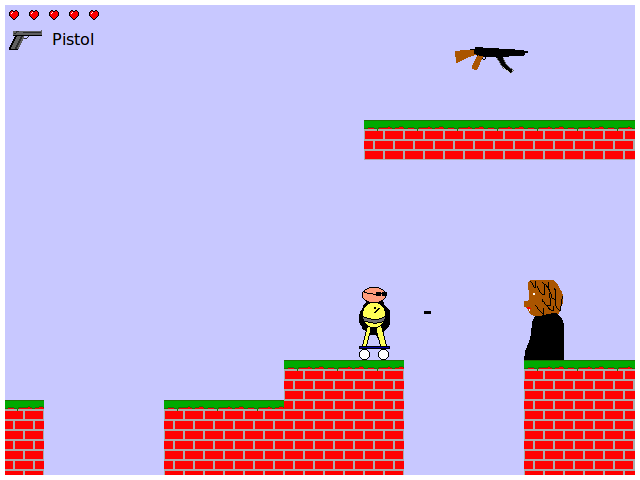
\includegraphics[width=11cm]{skarmdomp}
\caption{En typisk spelsituation.}\label{screenshot}
\end{figure}

Om spelaren dör så tar spelet slut och måste startas om för att kunna spelas igen. Målet med spelet är att ta sig till slutet av banan. 



\subsection{Kravlista}
Projektets kravlista återfinns i tabell \ref{kravlista} nedan.

\begin{table}[ht]
\rowcolors{2}{gray!25}{white}
	\caption{Kravlista}\label{kravlista}
	\centering
	\begin{tabular}{lp{8cm}rl}
	\toprule
		\# & Beskrivning & Prioritet &  \\
	\midrule
	1 & Spelet ska kunna styras med tangentbordet &
		1 & $\CheckedBox$ \\
	1.A & Spelaren ska kunna hoppa &
		1 & $\CheckedBox$ \\
	1.B & Spelaren ska kunna gå i sidled &
		1 & $\CheckedBox$ \\
	2 & Fiender skall finnas och vara möjliga att interagera med &
		1 & $\CheckedBox$ \\
	3 & Vapen skall kunna användas för att eliminera fiender &
		1 & $\CheckedBox$ \\
	4 & Banan skall innehålla olika hinder och objekt  &
		1 & $\CheckedBox$ \\
	5 & Man ska kunna klara spelet &
		2 & $\CheckedBox$ \\
	6 & Ett poängsystem, poäng fås av prylar och att döda fiender &
		3 & $\Box$ \\
	7 & Bakgrundsmiljön skall bestå av olika lager för att ge ett djup &
		3 & $\Box$ \\
	8 & En huvudmeny &
		3 & $\Box$ \\
	9 & En startskärm som inviger spelaren i sammanhanget &
		3 & $\Box$ \\
	10 & ”Hit points” &
		3 & $\CheckedBox$ \\
	11 & Extraliv &
		3 & $\Box$ \\
	12 & High scores &
		4 & $\Box$ \\
	13 & En boss skall finnas i slutet av banan &
		4 & $\Box$ \\
	14 & Flera banor &
		5 & $\Box$ \\
	15 & Power-ups: odödlighet, etc. &
		5 & $\Box$ \\
	16 & Musik &
		5 & $\Box$ \\

	\bottomrule
	\end{tabular}
\end{table}

\section{Implementation}
Det här kapitlet behandlar spelets implementation.

\subsection{Abstrakta datatyper}
\begin{adt-table}{\code{map\%} (bana)}{map-adt}
dump-tiles-to-file & filnamn & skickar vidare argumentet till tilemap  \\ 
 
colliding? & obj1, obj2 & returnerar sant om objekten överlappar varandra \\ 
 
colliding-bullets & obj & returnerar alla bullets som kolliderar med obj \\ 
 
colliding-characters & obj & returnerar alla characters som kolliderar med obj \\ 
 
colliding-items & obj & returnerar alla items som kolliderar med obj \\ 

colliding-in & lst, obj & returnerar alla element i lst som kolliderar med obj \\ 
 
overlapping-tiles & obj & returnerar en lista med alla koordinater (x . y) för tiles som obj överlappar \\ 
 
colliding-tiles & obj & returnerar \#t om obj överlappar en solid tile, annars \#f \\ 
 
get-next-tile-pixel & solid?, x, y, direction & Börjar på position (x,y) och går åt hållet direction tills den stöter på en solid eller tom (beroende på "solid?") tile eller tills banan tar slut. Returnerar x- eller y-koordinaten för den punkten (beroende på om den letade i x- eller y-led)\\ 
 
get-next-solid-pixel & x, y, direction & samma som get-next-tile-pixel fast kollar alltid efter solid tile \\

get-next-empty-pixel & x, y, direction & samma som get-next-tile-pixel fast kollar alltid efter tom tile \\

get-position-tile & x, y & returnerar värdet på en tile vid pixlar (x,y) \\

get-screen-position-tile & x, y & returnerar värdet på en tile vid pixlar (x,y) med x kompenserat för scrollning \\

solid-tile-at? & x, y & returnerar sant om givna pixelkoordinater är del av en solid tile \\

valid-tile-coord? & x, y & returnerar sant om x, y är giltiga koordinater för tiles \\

valid-tile-coord-at-screen? & x, y & returnerar sant om x, y konverterat till tile-koordinater är giltiga koordinater för tiles (x kompenseras för scrollning) \\

set-tile-at-screen! & x, y, value & ändrar tilen vid pixel-koordinater x, y till value med x kompenserat för scrollning \\

add-element! & element & lägger in ett element i banan\\

delete-element! & element & tar bort ett element från banan \\
update & - & uppdaterar alla characters och bullets på banan, uppdaterar positioner, kollar om spelaren har vunnit, justerar scrolled-distance, tar bort bullets som inte ska vara kvar \\
render & canvas, dc & ritar ut allting i banan \\
draw-rectangle & x, y, width, height, color, canvas, dc & ritar ut en rektangel med en viss färg och kompenserar i x-led för sidoscrollning \\
draw-bitmap & bitmap, x, y, canvas, dc & ritar ut en bitmap och kompenserar i x-led för sidoscrollning \\

\end{adt-table}

\begin{adt-table}{\code{character\%} (karaktär)}{karak-adt}
get-position & - & returnerar ett par med karaktärens x- och y-position \\

add- & item & lägger in föremålet i karaktärens inventarium \\

take-weapon! & weapon & gör vapnet aktuellt och lägger in vapnet i inventariet. \\

switch-weapon! & next/prev & roterar inventariet \\

shoot! & - & avfyrar aktuellt vapen \\

remove-self! & - & tar bort karaktären från banan \\

swap-direction & direction & byter karaktärens riktning \\

on-ground? & - & returnerar \#t om karaktären står på marken \\

find-obstacle & solid?, direction & returnerar en pixel-koordinat för en tom eller solid tile i riktningen direction \\

roof-y & - & Returnerar närmsta solida pixel-koordinat ovan karaktären.  \\

left-x & - & Returnerar närmsta solida pixel-koordinat till vänster om karaktären.  \\

right-x & - & Returnerar närmsta solida pixel-koordinat till höger om karaktären.  \\

ground-y & - & Returnerar närmsta solida pixel-koordinat under karaktären.  \\

decelerate! & - & Minskar karaktärens hastighet i x-led.  \\

gravitate! & - & Ökar karaktärens hastighet i y-led.  \\

push! & dvx, dvy & ändrar karaktärens hastighet i x- och/eller yled \\

jump! & - & Ger karaktären en negativ hastighet i y-led.  \\

render & canvas, dc & säger åt banan att rita en rektangel. \\

move! & - & bestämmer hur spelaren skall röra sig \\

die! & - & se remove-self! \\

hurt! & damage & skadar karaktären \\

update! & - & kör move! \\

\end{adt-table}

\begin{adt-table}{\code{tilemap\%} (brickkarta)}{tilemap-adt}

dump-tiles-to-file & filename & spara tiles-vectorn till en fil \\

load-tiles! & input & ladda in tiles från en vector eller en fil \\

valid-tile-coord? & x, y & returnerar \#t om koordinaterna är tillåtna \\

get-position-tile & x, y & returnerar den tile som finns på x, y \\

get-next-tile-pixel & se map\% & se map\% \\

render-tiles & dc xs,ys & ritar ut tiles på dc \\

render & canvas, dc, scrolled distance & ritar ut alla tiles som ska synas på skärmen \\ 
 
\end{adt-table}


\begin{adt-table}{\code{player\%} (spelare)}{spelar-adt}

set-key! & key, boolean & sätter key till boolean \\

get-key & key & returnerar \#t om key är nedtryckt \\

update! & - & avgör vad som händer varje frame \\

\end{adt-table}

\begin{adt-table}{\code{enemy\%} (fiende)}{fiende-adt}

left-x & - & returnerar närmsta pixelkoordinaten för antingen en solid tile eller en kant av en platå åt vänster \\

right-x & - & returnerar närmsta pixelkoordinaten för antingen en solid tile eller en kant av en platå åt höger \\

update! & - & avgör vad som händer varje frame \\

\end{adt-table}


\begin{adt-table}{\code{bullet\%} (kula)}{kula-adt}

remove-self & - & tar bort kulan från banan \\

render & canvas, dc & ritar kulan på banan \\

update! & - & kör move! \\

move & - & flyttar kulan \\

\end{adt-table}

\begin{adt-table}{\code{hud\%} (hud)}{hud-adt}

render & canvas, dc & ritar HUD:en på skärmen \\

\end{adt-table}

\begin{adt-table}{\code{weapon\%} (vapen)}{vapen-adt}

render & canvas, dc & ritar vapnet på skärmen  \\

fire! & the-map, direction & avlossar ett skott om vapnet befinner sig hos en spelare \\
 
\end{adt-table}
\subsection{Testning}
Testning kommer att kunna ske kontinuerligt under programmeringen. Hög prioritet ligger på att få till en fungerande spelmiljö, så att testningen kan börja så tidigt som möjligt. Om behov av speciella testfunktioner upptäcks implementeras dessa i stunden.

\subsection{Beskrivning av implementationen}
Spelet har programmerats objektorienterat vilket innebär att spelare, fiender och bana representeras av objekt. Eftersom koden för spelaren och fienderna har många gemensamma drag så har en karaktärsklass skapats, som båda dessa bygger på. Rackets inbyggda objektsystem har använts för de olika klasserna.

\subsubsection{Allmän kodstruktur}

Koden har delats upp så att varje klass ligger i en egen fil. I filen \textsl{main.scm} laddas all annan kod in. Här skapas spelaren, fienderna och banan etc. En timer som tickar 60 ggr/sekund styr hur ofta spellogiken skall uppdateras. 

\subsubsection{Banan}
En tile-map (brickkarta) har skapats för att användas som bana. Varje tile är 40x40 pixlar och kan antingen vara solid eller tom. Är den solid så krockar en karaktär med den och är den tom händer ingenting. Mark och hinder består följaktligen av en mängd tiles i olika formationer. Dessa tiles täcker hela banan och solida tiles kan ha olika utseende genom att de innehåller olika bitmaps (bilder).

Det är banan som säger åt allt som finns i den att rita sig genom att sända proceduranropet render till varje element på banan. 
 

\subsubsection{Karaktärer}

Karaktärsklassen är gemensam för fiender och spelare. Denna klass innehåller metoder som hanterar vad som ska hända när karaktären krockar med något, tar skada, tar upp och byter vapen etc.  

\subsubsection{Skott}

Skotten är objekt som kan avlossas från vapen. Dessa tas bort när de åker utanför den synliga delen av banan för att spara datorkapacitet. De tas även bort vid krock med solida tiles samt efter att ha träffat tex. en fiende. 

\section{Utvärdering och erfarenheter}

%Detta avsnittet är en väldigt viktig del av projektspecifikationen. Här ska ni %tänka tillbaka och utvärdera projektet (något som alltid ska göra efter ett %projekt). Som en hjälp på vägen kan ni utgå från följande frågeställningar:

\textbf{Vad gick bra? Mindre bra?}
Projektet har gått bra överlag och vi är nöjda med resultatet.  
\textbf{Lade ni ned för mycket/lite tid?}
Vi har inte lagt ned riktigt lika mycket tid som vi hade räknat med, ungefär 20 timmar mindre per person. Dock skulle jag (Magnus) inte vilja påstå att vi har lagt ner för lite tid, eftersom vi inte hade hunnit jobba så mycket mer på den utsatta tiden om vi inte hade suttit ännu mer på kvällar och helger.

\textbf{Var arbetsfördelningen jämn? Om inte: Vad hade ni kunnat göra för att förbättra den?}
Arbetsfördelningen var relativt jämn, dock så hann Rolf göra mer än Magnus på samma antal timmar arbete eftersom han är en mer erfaren programmerare. Vi jobbade tillsammans ganska länge innan vi delade upp kodandet, vilket kan ha medfört att vi i slutändan hann mindre totalt. Dock så kändes det bra att bygga upp grundstommen tillsammans. 

\textbf{Har ni haft någon nytta av specifikationen? Vad har varit mest användbart med den? Minst?}
Vi har i princip använt specifikationen till att titta på vår kravlista. Om vi hade funderat mer på hur vi tänkte lägga upp kodandet innan vi satte igång, och skrivit in våra tankar, hade vi förmodligen tittat mer på den, men vi båda kände att vi ville komma igång och använda oss av arbetssättet att fundera under arbetets gång vad som kunde behövas osv. Vi ville absolut inte låsa oss till vissa grejer (tex. bestämma precis vilka kontroller som skulle användas och hur karaktärerna skulle se ut) utan ville känna friheten att kunna ändra oss efterhand. 

\textbf{Har arbetet fungerat som ni tänkt er? Har ni följt arbetsmetodiken? Något som skiljer sig? Till det bättre? Till det sämre?}



\textbf{Vad har varit mest problematiskt, om man utesluter den programmeringstekniska delen? Alltså saker runt omkring, som att hitta ledig tid eller plats att vara på.}

\textbf{Vad har ni lärt er så här långt som kan vara bra att ta med till kommande kurser/projekt?} Vi har bland annatlärt oss att dela upp kodandet och samarbeta via versionhanteringssystemet git.

\section{Tidrapportering}
Rapportering av arbetstid har skett fortlöpande i ett separat dokument som finns på Google Drive.


\end{document}